\chapter{Datenanalyse und Modellbildung}
\label{chap:analyse}

In dieser Phase erfolgte die tiefergehende Untersuchung der Forschungsfrage nach den Risikofaktoren für Armut. Basierend auf den Erkenntnissen der Vorverarbeitung wurden nicht-parametrische Tests für Gruppenvergleiche und  multivariate Regressionsmodelle eingesetzt.

\section{Explorative Analyse der Berufsgruppen}
Um festzustellen, ob sich das Armutsrisiko zwischen den verschiedenen sozialen Sektionen signifikant unterscheidet, wurde ein Gruppenvergleich durchgeführt. Da die Voraussetzung der Normalverteilung verletzt war, wurde der \textbf{Kruskal-Wallis-Test} als nicht-parametrische Alternative zur ANOVA gewählt.

\begin{itemize}
    \item \textbf{Ergebnis:} Der Test lieferte eine Teststatistik von $H = 68,15$ bei einem p-Wert von $4,47 \times 10^{-08}$.
    \item \textbf{Interpretation:} Die Nullhypothese, dass die Armutsrate über alle Sektionen hinweg gleich verteilt ist, wurde abgelehnt. Es existieren somit hochsignifikante Unterschiede im Armutsrisiko zwischen den Berufsgruppen.
\end{itemize}

\section{Multivariate Modellierung der Risikofaktoren}
Um den Einfluss mehrerer Faktoren gleichzeitig zu isolieren, wurde eine multiple lineare Regression (OLS) berechnet. Hierbei wurden zwei Modelle verglichen, um die bestmögliche statistische Güte zu erreichen.

\subsubsection{Modellvergleich und Residuendiagnostik}
Ein zentrales Gütekriterium für Regressionsmodelle ist die Normalverteilung der Residuen.
\begin{itemize}
    \item \textbf{Basis-Modell:} Die Residuen des ursprünglichen Modells wiesen eine starke Abweichung von der Normalverteilung auf ($p = 4,59 \times 10^{-10}$).
    \item \textbf{Transformiertes Modell:} Durch eine Log-Transformation ($\log1p$) der Zielvariable \textit{poverty\_rate} konnte die Verteilung der Residuen signifikant verbessert werden (Teststatistik: 0,9842; $p = 0,001$).
\end{itemize}
Aufgrund dieser Ergebnisse wurde das transformierte Modell für die finale Interpretation gewählt, da es die statistischen Voraussetzungen besser erfüllt.

\subsubsection{Robustheit der Schätzung}
Um die Ergebnisse jenseits rein deskriptiver Zahlen abzusichern, wurde die Kovarianz-Matrix des Modells mit \textbf{robusten Standardfehlern (Typ HC3)} berechnet. Dieses Verfahren schützt die Signifikanztests vor Verzerrungen durch Heteroskedastizität, was angesichts der historischen Datenqualität eine notwendige methodische Absicherung darstellt.

\subsubsection{Zusammenfassung der Modellergebnisse}
Das finale Modell erreicht ein bereinigtes Bestimmtheitsmaß ($Adj. R^{2}$) von $0,192$. Dies bedeutet, dass ca. $19,2\%$ der Varianz der Armutsrate durch die einbezogenen Faktoren erklärt werden können. Sämtliche Koeffizienten wurden auf ihre Signifikanz geprüft, um belastbare Aussagen über die Risikofaktoren treffen zu können.

\begin{figure}[htpb!]
    \centering
    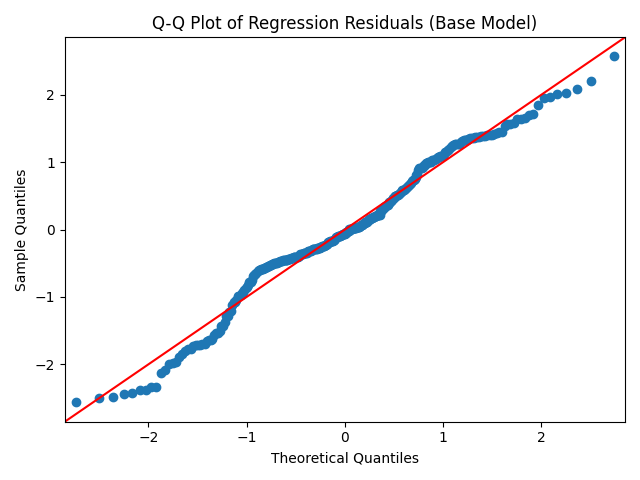
\includegraphics[width=0.65\textwidth]{contents/figures/regression_qqplot.png}
    \caption{regression-qqplot}
    \label{fig:regression1}
\end{figure}

\begin{figure}[htpb!]
    \centering
    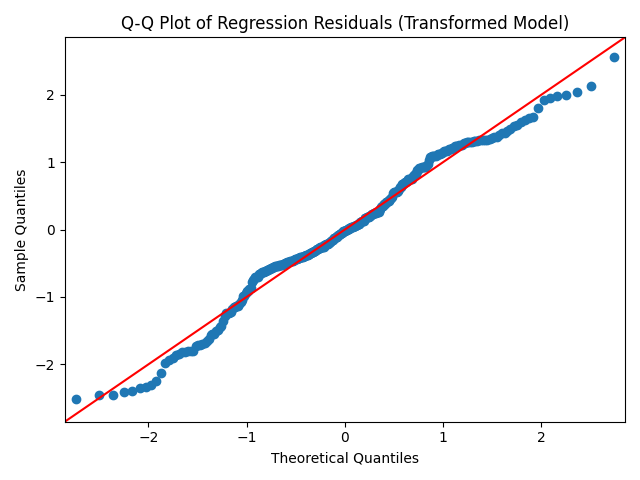
\includegraphics[width=1.1\textwidth]{contents/figures/transformed_model_qqplot.png}
    \caption{regression-qqplot2}
    \label{fig:regression3}
\end{figure}
